%%%%%%%%%%%%%
% LECTURE 2 %
%%%%%%%%%%%%%

\newpage
\noindent \lecture{2}{08/10/2021}

\section{Osservabili}\label{sec:osservabili}

\begin{itemize}
    \item \textbf{II Postulato} (\textbf{Osservabili}): Che cosa si può misurare in QM? Vengono misurate le \textbf{osservabili}, ossia \textbf{operatori autoaggiunti} (o \textbf{hermitiani}) $\hat{A}$ tali che
    \begin{equation*}
        \hat{A}: \mathcal{H}\rightarrow \mathcal{H} \, \text{ con } \, \hat{A}^\dagger = \hat{A} \, ,
    \end{equation*}
    dove più precisamente $\hat{A}^\dagger \equiv (\hat{A}^t)^\ast$. Dal punto di vista degli elementi di matrice, calcolare l'aggiunto di $A_{ij}$ significa $A^\dagger_{ij} = A^\ast_{ji}$. Dunque le matrici autoaggiunte (hermitiane) sono tali che $A^\dagger \equiv (A^t)^\ast = A$.  
\end{itemize}

\noindent In base a ciò che abbiamo visto sulla notazione braket  ($\bra{\phi} = \ket{\phi}^\dagger$) abbiamo necessariamente che

\begin{equation*}
    \ket{\psi} = B \ket{\phi} \, , \quad \Rightarrow \quad  \bra{\psi} = \bra{\phi} B^\dagger \, .
\end{equation*}

\noindent Focalizzando la nostra attenzione sugli operatori autoaggiunti, richiamiamo un importante teorema dell'algebra lineare:
\begin{teorema}[\textbf{Teorema Spettrale}]
    Sia $\hat{A}$ un operatore autoaggiunto su uno spazio di Hilbert $\mathcal{H}$ (reale o complesso). Allora esiste una base ortonormale di $\mathcal{H}$ composta da autovettori di $\hat{A}$, ossia $\exists$ $\lbrace \ket{n} \rbrace \in \mathcal{H}$ tale che $\hat{A} \ket{n} = a_n \ket{n}$ dove gli autovalori $a_n \in \mathbb{R}$.
\end{teorema}

\noindent Si noti dal teorema che $\braket{n}{m} = \delta_{nm}$ dove $n,m = 1, \ldots, N$ con $N \equiv \dim \mathcal{H}$. Trattandosi di una base, qualsiasi vettore dello spazio di Hilbert può essere scritto come combinazione lineare di tali vettori: 

\begin{equation*}
    \ket{\psi} = \sum_{n=1}^N \alpha_n \ket n \, , \, \text{ dove } \, \alpha_n \equiv \braket{n}{\psi} \in \mathbb{C} \, .
\end{equation*}

\noindent Ritornando al nostro caso del sistema a due livelli, lo spazio di Hilbert in esame è $\mathbb{C}^2$, dove consideriamo la \textbf{base canonica} (o \textbf{base computazionale}) data dagli stati $\ket 0$ e $\ket 1$ (si veda \eqref{computational_basis}). In questo spazio vettoriale gli operatori sono rappresentati da matrici $2 \times 2$. La più generale matrice $2 \times 2$ hermitiana contenente 4 parametri reali è

\begin{equation*}
    A = 
    \begin{pmatrix}
        a+b & c-id \\ 
        c+id & a-b
    \end{pmatrix} \, ,
\end{equation*}

\noindent dove $a, b, c, d \in \mathbb{R}$. Si noti che sulla diagonale le entrate sono puramente reali. Così come abbiamo decomposto uno stato generico $\ket{\psi}$ mediante combinazione lineare di autovettori $\ket{n}$, possiamo decomporre il generico operatore hermitiano di $\mathbb{C}^2$ come 

\begin{equation*}
    A = a \mathbb{I} + c \sigma_1 + d \sigma_2 + b \sigma_3 \, ,
\end{equation*}

\noindent dove $\mathbb{I}$ è la matrice \textbf{identità} e $\sigma_1, \sigma_2, \sigma_3$ sono le \textbf{matrici Pauli}:

\begin{equation}\label{Pauli_matrices}
    \sigma_1=
    \begin{pmatrix}
        0 & 1 \\
        1 & 0
    \end{pmatrix} \, , \ \ \ \ \
    \sigma_2=
    \begin{pmatrix}
        0 & -i \\
        i & 0
    \end{pmatrix} \, , \ \ \ \ \
    \sigma_3=
    \begin{pmatrix}
        1 & 0 \\
        0 & -1
    \end{pmatrix} \, . \ \ \ \ \
\end{equation}

\noindent Si ricordi che le matrici di Pauli sono i generatori del momento angolare in QM e sono infatti utilizzate per descrivere lo spin come $\hat{\vec{S}} = \frac{\hbar}{2} \hat{\vec{\sigma}}$. I relativi autovalori e autovettori sono mostrati nella tabella \ref{tab:Pauli_eig}.

\begin{table}[!ht]
	\centering
    \begin{tabular}{ccc}
        \toprule
        \textbf{Matrice di Pauli} & \textbf{Autovettori} & \textbf{Autovalori}  \\
        \midrule
        $\sigma_1$ & $\ket + = \frac{1}{\sqrt 2} \begin{pmatrix} 1 \\ 1 \end{pmatrix}, \qquad \ket - = \frac{1}{\sqrt 2} \begin{pmatrix} 1 \\ -1 \end{pmatrix} $ & $\lbrace 1, -1 \rbrace$ \\
        $\sigma_2$ & $\ket i = \frac{1}{\sqrt 2} \begin{pmatrix} 1 \\ i \end{pmatrix}, \qquad \ket{-i} = \frac{1}{\sqrt 2} \begin{pmatrix} 1 \\ -i \end{pmatrix} $ & $\lbrace 1, -1 \rbrace$ \\
        $\sigma_3$ & $\ket 0 = \begin{pmatrix} 1 \\ 0 \end{pmatrix}, \qquad \ket 1 = \begin{pmatrix} 0 \\ 1 \end{pmatrix} $ & $\lbrace 1,-1 \rbrace$ \\
        \bottomrule
    \end{tabular}\\
    \caption{Autovettori e autovalori delle matrici di Pauli.}
    \label{tab:Pauli_eig}
\end{table}

\noindent Dato che in futuro ci tornerà utile, osserviamo che gli autovettori di $\sigma_1$ e $\sigma_2$ possono essere espressi mediante base computazionale come

\begin{equation}\label{basi_di_sigma_12}
    \ket + = \frac{\ket 0 + \ket 1}{\sqrt 2} \, , \quad \ket - = \frac{\ket 0 - \ket 1}{\sqrt 2} \, , \quad \ket i = \frac{\ket 0 + i \ket 1}{\sqrt 2} \, , \quad \ket{-i} = \frac{\ket 0 - i \ket 1}{\sqrt 2} \, ,
\end{equation}

\noindent Utilizzando la rappresentazione dei qubit tramite sfera di Bloch, questi autovettori sono mostrati in figura \ref{fig:BlochSphere2}. 

\begin{figure}[!ht]
    \centering
    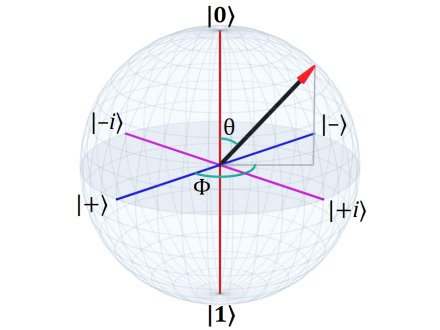
\includegraphics[scale=0.6]{images/bloch-hdr-440.png}
    \caption{Rappresentazione degli autovettori delle matrici di Pauli sulla sfera di Bloch. Il punto indicato dalla freccia rossa indica un generico qubit.}
    \label{fig:BlochSphere2}
\end{figure}

\noindent Come detto in precedenza, le 3 matrici di Pauli parametrizzano lo spin e i 3 assi della sfera di Bloch possono essere associati allo spin. Considerando lo stato generico $\ket{\psi}$ della \eqref{generic qubit}, possiamo definire lo spin lungo una direzione generica $\vec{\sigma} \cdot \vec{n}$ dove $\vec n = (\cos\phi\sin\theta, \sin\phi\sin\theta, \cos\theta)$:

\begin{equation*}
    \vec{\sigma} \cdot \vec n = \cos\phi\sin\theta \sigma_1 + \sin \phi \sin \theta \sigma_2 + \cos \theta_3 \, \, ;
\end{equation*}
così facendo è un semplice esercizio di QM dimostrare che $\ket{\psi}$ è autostato di $\vec{\sigma} \cdot \vec n$, ossia $\vec{\sigma} \cdot \vec n \ket{\psi} = \ket{\psi}$. Questo significa che dato uno stato sulla sfera di Bloch, allora è autostato dello spin nella direzione individuata da tale qubit: l'idea fisica alla base della sfera di Bloch è che la direzione arbitraria scelta non è altro che la direzione della quantizzazione dello spin. 

\section{Misurazioni}

\begin{itemize}
    \item \textbf{III Postulato} (\textbf{Regola di Born}):
    \begin{enumerate}
        \item \textbf{Misurazione}: sia $\hat{A}$ un osservabile con autostati $\ket{n}$, ossia $\hat{A} \ket{n} = a_n \ket{n}$. Prendiamo per semplicità $a_n \neq a_m \ \forall n \neq m$ (osservabile con autovalori distinti). Consideriamo uno stato generico espanso sugli autostati precedenti: $\ket \psi = \sum_n \alpha_n \ket n$. Allora una misura dell'osservabile $\hat{A}$ produce il valore $a_n$ con probabilità data da $\abs{\alpha_n}^2$ (assumendo lo stato correttamente normalizzato).
        
        \item \textbf{Collasso dello stato}: cosa succede allo stato del sistema dopo la misurazione? Istantaneamente lo stato $\ket \psi$ collassa sull'autostato associato all'autovalore risultante dalla misura. Ad esempio se misurando otteniamo $a_n$ allora $\ket{\psi} \rightarrow \ket{n}$. Effettuando delle misure successive sullo stato si ottiene sempre $\ket{n}$ con probabilità esattamente uguale a 1.  
    \end{enumerate}
\end{itemize}

\begin{esempio}
    Consideriamo per esempio il generico qubit \eqref{generic qubit} e immaginiamo di voler effettuare delle misurazioni in differenti basi. Supponiamo di voler misurare lo spin lungo $z$ (base $\lbrace \ket{0}, \ket{1} \rbrace$ di $\sigma_3$) e lungo $x$ (base $\lbrace \ket{+}, \ket{-} \rbrace$ di $\sigma_1$). Essendo il qubit già decomposto sulla base computazionale, una misurazione lungo $z$ produrrà
    
    \begin{equation*}
        P(\ket{0}) = \abs{\cos \! \left( \frac{\theta}{2} \right)}^2 \, , \qquad P(\ket{1}) = \abs{\sin \! \left( \frac{\theta}{2} \right)}^2 \, .
    \end{equation*}
    
    \noindent Per capire il risultato della misurazione lungo $x$, invece, dobbiamo espandere $\ket{\psi}$ sulla base $\lbrace \ket{+}, \ket{-} \rbrace$: usando le \eqref{basi_di_sigma_12} per esprimere $\lbrace \ket{0}, \ket{1} \rbrace$ in termini di $\lbrace \ket{+}, \ket{-} \rbrace$ ricaviamo
    
    \begin{equation*}
        P(\ket{+}) = \frac{1}{2} \abs{\cos \! \left( \frac{\theta}{2} \right) + e^{i \phi} \sin \! \left( \frac{\theta}{2} \right)}^2 \, , \qquad P(\ket{-}) = \frac{1}{2} \abs{\cos \! \left( \frac{\theta}{2} \right) - e^{i \phi} \sin \! \left( \frac{\theta}{2} \right)}^2 \, .
    \end{equation*}
    
    \noindent Si noti come in entrambe le situazioni la probabilità risulta correttamente normalizzata: $P(\ket{0}) + P(\ket{1}) = P(\ket{+}) + P(\ket{-}) = 1$. 
\end{esempio}

\begin{esempio}
    Consideriamo lo stato $\ket{+}$ delle \eqref{basi_di_sigma_12}. Qual è l'interpretazione fisica di tale stato? Supponiamo che rappresenti lo spin di una particella: quando lo spin si trova in $\ket{+}$ allora sappiamo con certezza che punta lungo la direzione $x$, ossia $P(\ket{+}) = 1$. Al contrario, per una misurazione lungo $z$ sappiamo che $P(\ket{0}) = 1/2$ e $P(\ket{1}) = 1/2$: abbiamo la certezza del risultato lungo le $x$, ma lungo le $z$ si ha totale incertezza. Questo fenomeno è dovuto alla non commutatività degli operatori di spin nelle 3 direzioni:
    
    \begin{equation*}
        \comm{\hat{S}_i}{\hat{S}_j} = i \hbar \varepsilon_{ijk} \hat{S}_k \, .
    \end{equation*}
    
    \noindent Se consideriamo infatti il sistema preparato in $\ket{+}$ e supponiamo di effettuare una misura lungo $z$ ottenendo $\ket{0}$ allora lo stato collasserà in $\ket{0}$ e, d'ora in avanti, qualsiasi misurazione lungo $z$ produrrà sempre $\ket{0}$ con $P(\ket{0}) = 1$. Nonostante ciò, il fatto che $\hat{S}_z$ non commuti con $\hat{S}_x$ fa sì che una misura successiva lungo $x$ "rigeneri" dell'incertezza: $P(\ket{+}) = 1/2$ e $P(\ket{-}) = 1/2$ (si veda $\ket{0}$ espresso in termini di $\lbrace \ket{+}, \ket{-} \rbrace$ dalle \eqref{basi_di_sigma_12}). 
\end{esempio}

\noindent Discutiamo la generalizzazione del III postulato nel caso in cui alcuni autovalori associati ad autostati differenti siano uguali, ovvero in presenza di \textbf{degenerazione}. Per esempio supponiamo il caso $N = \dim \mathcal{H} = 6$: 

\begin{equation*}
    \ket \psi = \alpha_1 \ket 1 + \alpha_2 \ket 2 + \alpha_3 \ket 3 + \alpha_4 \ket 4 + \alpha_5 \ket 5 \alpha_6 \ket 6 \, , 
\end{equation*}

\noindent dove supponiamo la degenerazione su $a_1 = a_2$ e $a_4 = a_5 = a_6$. Introduciamo gli operatori $\hat{P}_{a_i}$ che considerano solamente la parte di $\ket{\psi}$ corrispondente all'autospazio associato ad $a_i$:

\begin{equation*}
    \ket \psi = \underbrace{\alpha_1 \ket 1 + \alpha_2 \ket 2 }_{\hat P_{a_1} \ket \psi} + \underbrace{\alpha_3 \ket 3}_{\hat P_{a_3} \ket \psi} + \underbrace{\alpha_4 \ket 4 + \alpha_5 \ket 5 + \alpha_6 \ket 6}_{\hat P_{a_4 \ket \psi}} \, ;
\end{equation*}

\noindent tali operatori prendono il nome di \textbf{proiettori} e soddisfano le proprietà seguenti:  
\begin{enumerate}
    \item $\hat P_{a_i}^\dagger = \hat P_{a_i}$.
    \item $\hat P_{a_i}^2 = \hat P_{a_i}$. 
    \item $\sum_i \hat P_{a_i} = \mathbb{I}$. 
\end{enumerate}

\noindent I proiettori sono utili per scrivere la \textbf{regola di Born} (III postulato) nel caso generale: dato uno stato $\ket{\psi}$ con degenerazione sugli autovalori $a_i$, la probabilità di ottenere il risultato $a_n$ è

\begin{equation*}
    P(a_n) = \norm{\hat{P}_{a_n} \ket{\psi}}^2 \, ;
\end{equation*}

\noindent dopo la misura la funzione d'onda collassa sul seguente stato normalizzato:

\begin{equation*}
    \ket{\psi} \rightarrow \frac{\hat{P}_{a_n} \ket{\psi}}{\norm{\hat{P}_{a_n} \ket{\psi}}} \, .
\end{equation*}

\noindent Ad esempio, nel caso dello stato sopra scritto, la probabilità di ottenere $a_1 = a_2$ non è altro che 

\begin{equation*}
    P(a_1) = \norm{\hat{P}_{a_1} \ket{\psi}}^2 = \norm{\alpha_1 \ket{1} + \alpha_2 \ket{2}}^2 = \abs{\alpha_1}^2 + \abs{\alpha_2}^2 \, ,
\end{equation*}

\noindent e lo stato collassa su

\begin{equation*}
    \ket{\psi} \rightarrow \frac{\alpha_1 \ket{1} + \alpha_2 \ket{2}}{\sqrt{\abs{\alpha_1}^2 + \abs{\alpha_2}^2}} \, ;
\end{equation*}

\noindent ora si ha incertezza su quale stato si trova $\ket{\psi}$, ma con un esperimento successivo siamo in grado di risolvere la degenerazione e ottenere $\ket{1}$ o $\ket{2}$. 

\section{Evoluzione temporale}
Il postulato successivo riguarda l'evoluzione temporale degli stati:

\begin{itemize}
    \item \textbf{IV Postulato} (\textbf{Evoluzione temporale}): L'evoluzione temporale di uno stato generico $\ket{\psi(0)}$ è descritta dall'equazione di Schrödinger:
    
    \begin{equation*}
        i \hbar \dv{t} \ket{\psi(t)} = \hat H \ket{\psi(t)} \, ,
    \end{equation*}
    
    \noindent dove $\hat{H}$ è l'operatore (hermitiano) \textbf{hamiltoniana} del sistema. L'equazione di Schrödinger conserva le probabilità: $\braket{\psi(t)} = \braket{\psi(0)} = 1$. 
\end{itemize}

\noindent Solitamente si risolve questa equazione introducendo l'\textbf{operatore di evoluzione temporale} $\hat{U}(t)$:

\begin{equation*}
    \ket{\psi(t)} = \hat{U}(t) \ket{\psi(0)} \, ;
\end{equation*}

\noindent quando l'hamiltoniana è indipendente dal tempo $\hat{U}(t)$ diventa semplicemente

\begin{equation*}
    \hat{U} (t) = e^{-\frac{i}{\hbar} \hat H t} \, ;
\end{equation*}

\noindent se invece $\hat H = \hat H(t)$, è necessario distinguere i casi di hamiltoniane commutanti o non commutanti a tempi differenti.\\
\noindent Come detto sopra, l'evoluzione temporale preserva le probabilità e ciò è una diretta conseguenza del fatto che $\hat{U}(t)$ sia \textbf{unitario}: 
\begin{itemize}
    \item $\hat U \hat U^\dagger = \hat U^\dagger U = \mathbb{I} \quad \Rightarrow \quad \hat{U}^\dagger = \hat{U}^{-1}$.
    \item Il prodotto scalare è conservato: $\braket{\hat U\phi}{\hat U\psi} = \braket{\phi}{\hat U^\dagger \hat U\psi} = \braket{\phi}{\psi}$. 
\end{itemize}
\noindent Notiamo che $\hat{U}(t)$ per hamiltoniane indipendenti da $t$ è effettivamente unitario:

\begin{equation*}
    \hat U^\dagger \hat U = \left( e^{-\frac{i}{\hbar} \hat H t} \right)^\dagger e^{-\frac{i}{\hbar} \hat H t} = e^{\frac{i}{\hbar} \hat H t} e^{-\frac{i}{\hbar} \hat H t} = \mathbb{I} \, .
\end{equation*}

\section{Gate}\label{sec:gate}

\begin{definizione}[\textbf{Porte quantistiche}]
    L'analogo quantistico delle porte (o gate) logiche classiche sono le \textbf{porte quantistiche} (o \textbf{gate quantistici}). Un gate quantistico è un operatore unitario che cambia lo stato del sistema.
\end{definizione}

\noindent Notiamo che una delle principali differenze che rendono di difficile implementazione le porte quantistiche risiede nel fatto che non possiamo implementare direttamente le più semplici operazioni classiche come \texttt{AND}, \texttt{OR} o \texttt{XOR}. 

\begin{definizione}[\textbf{Circuito Quantistico}]
    Un \textbf{circuito quantistico} è un modello di computazione quantistica in cui una sequenza ordinata di gate quantistici è applicata ai qubit.
\end{definizione}

\noindent In un circuito classico l'uso dei gate logici è banale. Supponiamo di considerare un bit che si trova in 0 o 1: un gate costituisce l'implementazione di un agente esterno che cambia lo stato del bit. Si pensi ad esempio al gate \texttt{NOT} per il quale $a \rightarrow$ \texttt{NOT} $a$:
\newline
\begin{center}
    \begin{circuitikz}
        \draw
        (0,4.5) node[not port] (mynot) {}
        (mynot.in) node[left = .4cm, anchor=east] (a) {$0$}
        (mynot.out) node[right = .4cm,anchor=west] (b) {$1 \, ,$}
        (mynot.in) -- (a)
        (mynot.out) -- (b);
    \end{circuitikz}
    \begin{circuitikz}
        \draw
        (0,4.5) node[not port] (mynot) {}
        (mynot.in) node[left = .4cm, anchor=east] (a) {$1$}
        (mynot.out) node[right = .4cm,anchor=west] (b) {$0 \, ,$}
        (mynot.in) -- (a)
        (mynot.out) -- (b);
    \end{circuitikz}
\end{center}

\noindent Nel caso invece di un qubit i circuiti funzionano diversamente perché le porte agiscono su sistemi a due livelli. Immaginiamo che a causa di un agente esterno il qubit $\ket{\psi}$ subisca un evoluzione temporale $\hat{U}$: rappresentiamo questo fatto mediante il circuito seguente
\begin{center}
    \mbox{
        \Qcircuit @C=2em @R=2em {
            \lstick{\ket{\psi}} & \gate{\hat{U}} & \rstick{\hat{U} \ket{\psi} \, ,} \qw \\
        }
    }
\end{center}

\noindent Si ricordi che $\hat{U}$ è sempre un operatore unitario: ad esempio per un'hamiltoniana indipendente dal tempo si ha semplicemente $\hat{U}(t) = e^{-\frac{i}{\hbar}\hat H t}$. \\
\noindent Consideriamo le matrici di Pauli: sappiamo che sono hermitiane ($\sigma^\dagger_i = \sigma_i$) e che soddisfano la proprietà $\sigma_i^2 = \mathbb{I}$, ma questo significa che sono anche matrici unitarie. Questo fatto ci permette di costruire\footnote{Un tale sistema in natura è abbastanza semplice da implementare poiché, essendo $\hat{H} = \vec{\sigma} \cdot \vec B$ l'accoppiamento tra spin e campo magnetico, è facile costruire una tale evoluzione temporale.} dei gate in cui $\hat{U} = \hat{\sigma}_i$.  Ad esempio è possibile implementare dei gate come $\mathbb{I}$, $\sigma_1 \equiv X$, $\sigma_2 \equiv Y$ e $\sigma_2 \equiv Z$. Ricordando che $\sigma_i \sigma_j = 2i \varepsilon_{ijk} \sigma_k$, notiamo che $XZ = - i Y$ e inoltre anche la matrice $-iY$ è unitaria. Per tale ragione molto spesso, al posto di considerare i gate $\lbrace \mathbb{I}, X, Y, Z \rbrace$ si sceglie la base $\lbrace \mathbb{I}, X, Z, XZ \rbrace$: questo significa che possiamo implementare i gate seguenti
\begin{center}
    \mbox{
        \Qcircuit @C=2em @R=2em {
            & \gate{X} & \qw \\
        }
    } 
    , \ \ \ \ 
    \mbox{
        \Qcircuit @C=2em @R=2em {
            & \gate{Z} & \qw \\
        }
    }
    , \ \ \ \ 
    \mbox{
        \Qcircuit @C=2em @R=2em {
            & \gate{XZ} & \qw \\
        }
    }
    ,
\end{center}

\noindent Consideriamo l'\texttt{X-gate}: dalle \eqref{Pauli_matrices} è evidente che $X$ rappresenta una sorta di "quantum" \texttt{NOT} perché inverte semplicemente lo stato della base computazionale:
\begin{center}
    \mbox{
        \Qcircuit @C=2em @R=2em {
            \lstick{\ket{0}} & \gate{X} & \rstick{\ket{1} \, ,} \qw \\
        }
    } 
    \\
    \mbox{
        \Qcircuit @C=2em @R=2em {
            \lstick{\ket{1}} & \gate{X} & \rstick{\ket{0} \, ,} \qw \\
        }
    }
\end{center}

\noindent Consideriamo ora lo \texttt{Z-gate}: gli stati della base computazionale sono autovettori con autovalori 0 e 1 di $\sigma_3$, quindi questo gate inverte semplicemente il segno
\begin{center}
    \mbox{
        \Qcircuit @C=2em @R=2em {
            \lstick{\ket{0}} & \gate{Z} & \rstick{\ket{0} \, ,} \qw \\
        }
    } 
    \\
    \mbox{
        \Qcircuit @C=2em @R=2em {
            \lstick{\ket{1}} & \gate{Z} & \rstick{-\ket{1} \, ,} \qw \\
        }
    }
\end{center}
L'azione dello \texttt{Z-gate} su un generico qubit risulterà quindi in
\begin{center}
    \mbox{
        \Qcircuit @C=2em @R=2em {
            \lstick{a \ket{0} + b \ket{1}} & \gate{Z} & \rstick{a \ket{0} - b \ket{1} \, ,} \qw \\
        }
    } 
\end{center}
e questo significa che $Z$ aggiunge semplicemente una fase $e^{i \pi} = -1$ allo stato. Ricapitolando: l'\texttt{X-gate} implementa un'interferenza dall'esterno che inverte lo stato (ad esempio cambia segno dello spin lungo $x$) e lo \texttt{Z-gate} implementa l'introduzione di una fase. \\
\noindent Una matrice particolarmente importante per i nostri scopi è 
\begin{equation}\label{Hadamard_matrix}
    H = \frac{1}{\sqrt{2}} 
    \begin{pmatrix}
        1 & 1 \\ 1 & -1 
    \end{pmatrix} \, , 
\end{equation}
chiamata \textbf{matrice di Hadamard}. Notiamo che è unitaria in quanto $H^\dagger H = \mathbb{I}$. Essa può essere implementata nel cosiddetto \texttt{H-gate} o \textbf{gate di Hadamard}: si tratta di un gate particolarmente importante (lo useremo largamente durante tutto il corso) in quanto permette di cambiare base $\lbrace \ket{0}, \ket{1} \rbrace \leftrightarrow \lbrace \ket{+}, \ket{-} \rbrace$ 

\begin{center}
    \mbox{
        \Qcircuit @C=2em @R=2em {
            \lstick{\ket{0}} & \gate{H} & \rstick{\ket{+} \, ,} \qw \\
        }
        \ \ \ \ \ \ \ \ \ \ \ \ \ \ \ \ \ \ \ \ 
        \Qcircuit @C=2em @R=2em {
            \lstick{\ket{+}} & \gate{H} & \rstick{\ket{0}\, ,} \qw \\
        }
    }
    \\
    \mbox{
        \Qcircuit @C=2em @R=2em {
            \lstick{\ket{1}} & \gate{H} & \rstick{\ket{-} \, ,} \qw \\
        } 
        \ \ \ \ \ \ \ \ \ \ \ \ \ \ \ \ \ \ \ \ 
        \Qcircuit @C=2em @R=2em {
            \lstick{\ket{-}} & \gate{H} & \rstick{\ket{1} \, ,} \qw \\
        }
    }
\end{center}

\noindent Possiamo introdurre anche le matrici seguenti (ci serviranno più avanti)

\begin{equation}\label{S_T_matrices}
    S \equiv \sqrt{Z} =
\begin{pmatrix}
    1 & 0 \\ 0 & i
\end{pmatrix} \, , \qquad 
T \equiv \sqrt{S} =
\begin{pmatrix}
    1 & 0 \\ 0 & e^{i \frac{\pi}{4}}
\end{pmatrix} \, ,
\end{equation}

\noindent Le matrici introdotte in precedenza costituiscono gli oggetti base con cui andremo a implementare diversi gate e circuiti durante tutto il corso. Per costruire il gate più generale possiamo esponenziare scrivendo $U = e^{-\frac{i}{\hbar} H t}$ dove $H = a \mathbb{I} + b_i \sigma_i$ e $a, b_i \in \mathbb{R}$ con $i = 1,2,3$. In particolare esiste una particolare classe di operatori che utilizzeremo molto
\begin{equation*}
    R_{\vec{n}} = e^{-i \frac{\lambda}{2} (\vec n \cdot \vec \sigma)} \, ;
\end{equation*}
si tratta di un caso particolare dell'esponenziazione precedente in cui $a = 0$ e i coefficienti $b_i$ sono scelti lungo un particolare versore $\vec n$. Questo operatore unitario implementa una rotazione di angolo $\lambda$ in una direzione particolare individuata da $\vec n$:

\begin{equation}\label{rotation_n_lambda}
    R_{\vec{n}} = e^{-i \frac{\lambda}{2} (\vec n \cdot \vec \sigma)} = \cos \! \left( \frac{\lambda}{2} \right) \mathbb{I} - i \sin \! \left( \frac{\lambda}{2} \right) \vec \sigma \cdot \vec n \, ;
\end{equation}
(si espanda il LHS con la serie di Taylor dell'esponenziale e si usi $(\vec \sigma \cdot \vec n)^2 = \mathbb{I}$ per dimostrare l'uguaglianza con il RHS). È possibile dimostrare, inoltre, che qualsiasi matrice unitaria $2 \times 2$ può essere scritta nella forma seguente
\begin{equation}\label{general_2by2_matrix}
    U = e^{i \alpha}
    \begin{pmatrix}
        e^{-i \frac{\beta}{2}} & 0 \\ 0 & e^{i \frac{\beta}{2}}
    \end{pmatrix}
    \begin{pmatrix}
        \cos \frac{\gamma}{2} & - \sin \frac{\gamma}{2} \\ \sin  \frac{\gamma}{2} & \cos \frac{\gamma}{2}
    \end{pmatrix}
    \begin{pmatrix}
        e^{-i \frac{\delta}{2}} & 0 \\ 0 & e^{i \frac{\delta}{2}}
    \end{pmatrix}
    = e^{i \alpha} R_z(\beta) R_x(\gamma) R_z(\delta) \, ; 
\end{equation}
perciò il più generale operatore unitario presenta 4 parametri reali $\alpha, \beta, \gamma, \delta \in \mathbb{R}$ e può implementare un possibile gate in un computer quantistico. Appare subito evidente come la scelta di 4 possibili parametri reali sia molto maggiore che nel caso dei gate logici classici. 